\section{Response of epipelagic community to extreme El Niño events}

This section details the simulated response of epipelagic communities to ENSO as a function of their size class and analyses the underlying mechanisms. Here, we focus on  analyzing the marine ecosystem response to the three strongest El Niño events in the historical record, namely those of 1982/83, 1997/98 and 2015/16 \citep{santosoDefiningCharacteristicsENSO2017}. During these events, the central and eastern Pacific warms by more than 2°C (Fig\ref{fig:nemo-had-sst}a), moving the warmest waters and related atmospheric convection from the western to the central Pacific. This atmospheric signature of El Niño has had dramatic climatic consequences, including droughts and wildfires in countries bordering the western Pacific, but also torrential rains and flooding along the south American coast (Cai et al. 2020). Its oceanic signature also tremendously impacted marine ecosystems and biodiversity, leading to major disruption of marine life and bird populations (Valle et al. 1987), promoting large-scale marine heatwaves (Hoolbrook et al. 2020) and coral bleaching (Clarr et al. 2018).  The response of the ocean during each of these three extreme events has been extensively described and analyzed in terms of physics  (e.g. Philander and Seigel 1985, \citealt{lengaigneOceanResponseMarch2002}, Puy et al. 2019), biogeochemistry (e.g. Barber and Chavez 1983, \citep{chavezBiologicalChemicalResponse1999}, Stramma et al. 2016) and marine ecosystems (Glynn et al. 1988, \citep{glynnCoralBleachingMortality2001}, Eakin et al. 2019). 

In order to isolate the generic response of epipelagic communities to extreme El Nino events, independent of the intrinsic characteritics of each event, we perform a composite analysis of these three extreme events, averaging monthly anomalies in temperature, ocean velocity, LTL concentrations and epipelagic commnunity biomass over the periods 1982-1984, 1997-1999 and 2015-2017. These extreme El Niño events are also followed by La Niña conditions the following year (more intense in the case of the 1997/98), also allowing for a discussion on the mechanisms driving the epipelagic community response to La Niña events. Although the temporal evolution and amplitude of the processes discussed below vary slightly between events, the relative importance of the processes discussed in our composite analysis remains the same when these three extreme events are analyzed individually (not shown). 

\subsection{Modeled upper-ocean response: from physics to ecosystems}

Because these are major environmental drivers of the epipelagic communities, we first describe in Figure \ref{fig:hov_nemo_ape}a-c the temporal evolution of monthly equatorial anomalies in upper ocean temperature, chlorophyll concentrations and zonal currents during and after extreme El Niño events, in the form of equatorial time-longitude diagrams. The warming signal associated with El Niño begins in the central equatorial Pacific in early spring, rapidly spreading to the eastern Pacific, intensifying during summer and fall, peaking at the end of the calendar year, and finally rapidly decreasing and transitioning to La Niña conditions the following spring (month 16, Fig.\ref{fig:hov_nemo_ape}a). The development phase of El Niño is also characterized by strong  eastward surface currents anomalies in the western and central Pacific (Figure \ref{fig:hov_nemo_ape}c) induced by anomalous westerly winds, favoring the central Pacific warming and eastward shift of the warm-pool towards the eastern equatorial Pacific. These current anomalies reverse at the peak of the El Niño and during La Niña. The simulated plankton concentration anomalies largely reflect those of temperature, with a strong decline during El Niño and an enhanced bloom during La Niña (Figure \ref{fig:hov_nemo_ape}.b). 


\begin{figure}[h!tp]
	\centering
	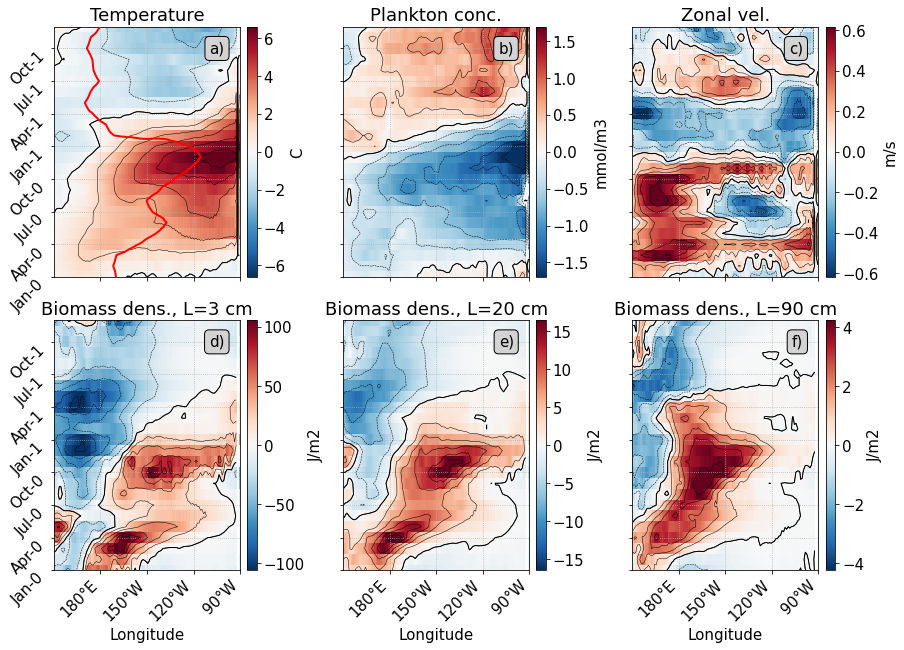
\includegraphics[scale=0.4]{plot_all_hovmoller_phys_oope.png}	
	\caption{Hovmoller diagrams of equatorial temperature (a), low-trophic level concentrations (b), zonal velocity (c) and fish biomass anomalies (3cm, 20cm and 90 cm in d, e, f, respectively).}	
	\label{fig:hov_nemo_ape}
\end{figure}

A similar analysis is then performed for epipelagic biomass for the three targeted size classes (Fig\ref{fig:hov_nemo_ape}d, Fig\ref{fig:hov_nemo_ape}e and Fig\ref{fig:hov_nemo_ape}f). Their response to El Niño has some common characteristics: positive biomass anomalies appear near the dateline early in the calendar year and propagate eastward toward the central Pacific until the end of spring (May/June). This positive anomaly in the central Pacific re-intensifies in fall and quickly disappears in winter. These positive anomalies east of the dateline are also accompanied by a decrease in biomass in the western Pacific starting in summer of the El Niño year. These negative anomalies persist after the El Niño peak and during the subsequent La Niña event but remain largely confined to the western Pacific. The behaviour of the three size classes, however,  shows significant differences, including an westward shifted response as the class size increases.

Our numerical tool allows us to extract the dominant processes responsible for the response of the epipelagic communities to El Niño represented on Figure \ref{fig:hov_nemo_ape} by analysing the associated tendency terms (equation ??). To do this, the same hovmuller diagrams are performed for the major tendency terms (right-hand side members of \ref{eq:apecosm_trend}) and their integral, representing their contribution to the total biomass change. We also aalyze various key parameters of the biological response to changes in the environmental conditions, namely the growth rate ($\gamma$ in equation \ref{eq:apecosm_trend}), the functional response and the predation mortality rates ($M$ in equation \ref{eq:apecosm_trend}). Because the relative importance of these processes varies with the size classes, these analyses are discussed separately for each size class.

\subsection{Processes driving epipelagic upper-ocean response}

Figure\ref{fig:fig7} presents a synthesis of the respective contribution of biological processes (i.e. the combined action of growth and predation) and physical processes (i.e. the combined action of advection and diffusion) on the epipelagic biomass response to ENSO as a function of their size class. For the largest size classes, physical processes (Fig\ref{fig:fig7}i) explain most of the biomass changes (Fig\ref{fig:fig7}g), with biological processes being an order of magnitude smaller (Fig\ref{fig:fig7}h). This dynamical response can be explained as follows: the strong eastward current anomalies in the western and central Pacific simulated during the onset and development phase of extreme El Niño (up to 0.6m/s; see Fig\ref{fig:hov_nemo_ape}c) tend to passively advect biomass of large epipelagic communities from the western Pacific to the central Pacific, explaining the increase in biomass in the central Pacific and its decrease in the west. While the influence of horizontal advection is broadly similar for all size classes, acting to increase fish biomass in the central Pacific under the action of strong eastward flowing currents, the relative importance of biological processes increases as the fish sizes decrease. For intermediate and small size classes, the decrease in biomass in the western Pacific is indeed primarily the result of biological processes. In the central and eastern Pacific, the combined action of dynamical and biological processes explain biomass increase during El Niño growth (Fig\ref{fig:fig7}a-f), while these processes largely cancel each other when the equatorial Pacific reverses to La Niña conditions, resulting in small biomass changes in this region.  


\begin{figure}[h!tp]
	\centering
	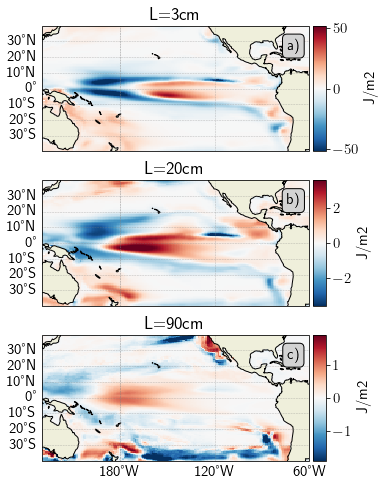
\includegraphics[scale=0.4]{figs/fig7.png}	
	\caption{Total (left), biologically (predation and growth, middle) and dynamically (right, advection and diffusion) induced changes in fish biomass for small (top), intermediate (middle) and large (bottom) sizes.}
	\label{fig:fig7}
\end{figure}

The influence of dynamical processes can easily be understood as the results of passive transport of fish biomass for all classes from the western to the central Pacific by strong eastward currents anomalies induced by extreme El Niño conditions. The significant and sometimes dominant contribution of biological processes for small and medium size classes, however, is more difficult to understand intuitively as it is the result of the combined action of predation and growth. Therefore, we further detail the respective contribution of predation and growth and their driving factors for small and medium size classes on Figures\ref{fig:fig8} and \ref{fig:fig9} respectively. For small size classes, predation and growth balance to first order (Fig.\ref{fig:fig8}a and Fig.\ref{fig:fig8}.b), resulting in a two- to threefold smaller net effect of biological processes (Fig. \ref{fig:hov_nemo_ape}d). Growth processes induce an increase  of biomass in the central Pacific (between dateline and 150\degree{}W) at the onset of El Niño, expanding eastward until its peak. These positive biomass anomalies then decrease slightly during the following La Niña conditions. This evolution can easily be related to the evolution of the modeled growth rate, which increases in the central and eastern Pacific during El Niño conditions and decrease slightly during the following La Niña conditions. These anomalous growth rate changes closely resembles the temperature evolution, indicating that changes in growth rate are largely temperature driven: i.e., the anomalous warming observed east of the dateline during El Niño increase growth rate and thus biomass of small size classes. The cooling observed during the subsequent La Niña conditions then decrease this growth rate, thereby damping the El Niño-induced increase in biomass. In contrast to the central and eastern Pacific, growth processes contribute to a decrease in biomass in the western Pacific from June of the El Niño year, which then intensifies during the following La Niña. Again, this decrease can directly related to the decrease in growth rate in the western Pacific driven by the cooling simulated in the western Pacific during the developping El Niño and the subsequent La Niña. The functional response is indeed not the main driver here, as its influence opposes the changes induced by growth processes: this functional response, which depends both on temperature and food density, show negative anomalies which are consistent with the reduction of low-trophic concentrations, hence suggesting a dominance of food density on the functional response. As mentioned earlier, changes in biomass induced by predation processes largely mirrors those induced by growth processes: they indeed act to decrease biomass in the central and eastern Pacific and increase it in the western Pacific. This response can directly be related to mortality rate through predation, which closely follow changes in larger fish biomass: the increase in biomass for intermediate size classes in the central Pacific acts to increase the mortality of smaller fishes through predation, the opposite happening in the western Pacific. Despite their opposite effect on biomass, growth processes overall dominates over predatation processes, explaining most of the decrease in biomass over the western Pacific during El Niño and the subsequent La Niña and enhancing the increase in biomass over the central Pacific induced by dynamical processes during El Niño.  

\begin{figure}[h!tp]
	\centering
	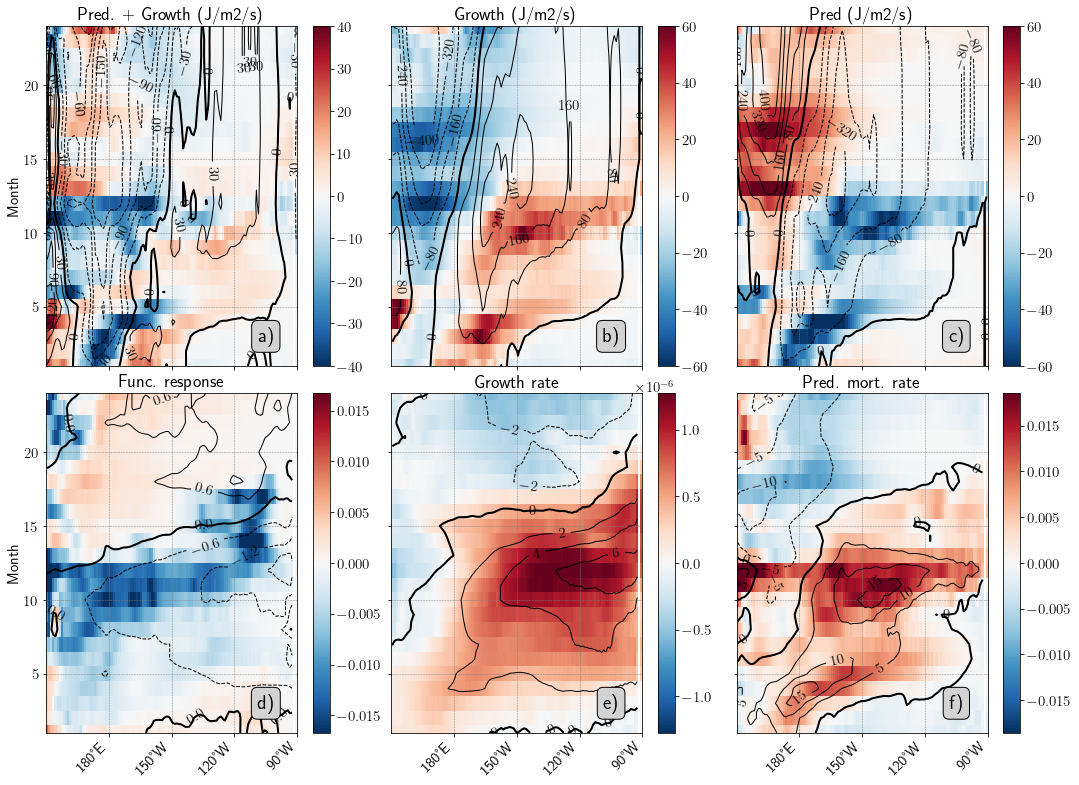
\includegraphics[scale=0.4]{figs/fig8.png}	
	\caption{Small sizes trends (colors) and time-integrated trends (contours) for growth and predation (a and b). Growth rate (colors) and temperature (contours) anomalies (c). Predation mortality rate (colors) and intermediate biomass anomalies (d). Functional response (colors) and plankton (contours) anomalies (f).}
	\label{fig:fig8}
\end{figure}

Changes in biomass induced by growth and predation processes for intermediate size classes display a similar evolution compared to those simulated for small size classes: they are opposite and of the same order of magnitudes but growth processes overall dominates over those from predation. Growth processes act to increase fish biomass in central Pacific from the onset to the peak of El Niño, while they decrease biomass in the western Pacific during the subsequent La Niña. However the influence of temperature changes on fish physiology is not anymore dominant factor contributing to biomass change from biological processes for intermediate size classes as it was the case for small individuals. As opposed to small size classes, growth rate changes large mirror changes in the functional response: functional response increases in the central Pacific because of both warmer temperatures and increase food availability provided by the increase of smaller size biomass, hence promoting an enhanced biomass growth the intermediate classes. IN THE WESTERN PACIFIC ???. Predation processes generally act to damp the effect of growth, reducing biomass in the central Pacific because of increased predation by large size classes there and increasing biomass in the western Pacific during the subsequent La Niña because of reduced predation. The changes induced by the combination of both processes is dominated by growth processes and resembles the one obtained for small sizes albeit a modest westward shift. As for small sizes, the biomass decrease in the western Pacific during El Niño and the subsequent La Niña is largely driven by a growth reduction, while dynamical processes dominate the biomass increase east of the dateline with a smaller contribution from growth.  The comparison of active and passive velocities suggest that passive movements (i.e. advection by the ocean currents) dominate, with ocean current anomalies greater than active velocity anomalies by a factor of $\approx\ 20$.

\begin{figure}[h!tp]
	\centering
	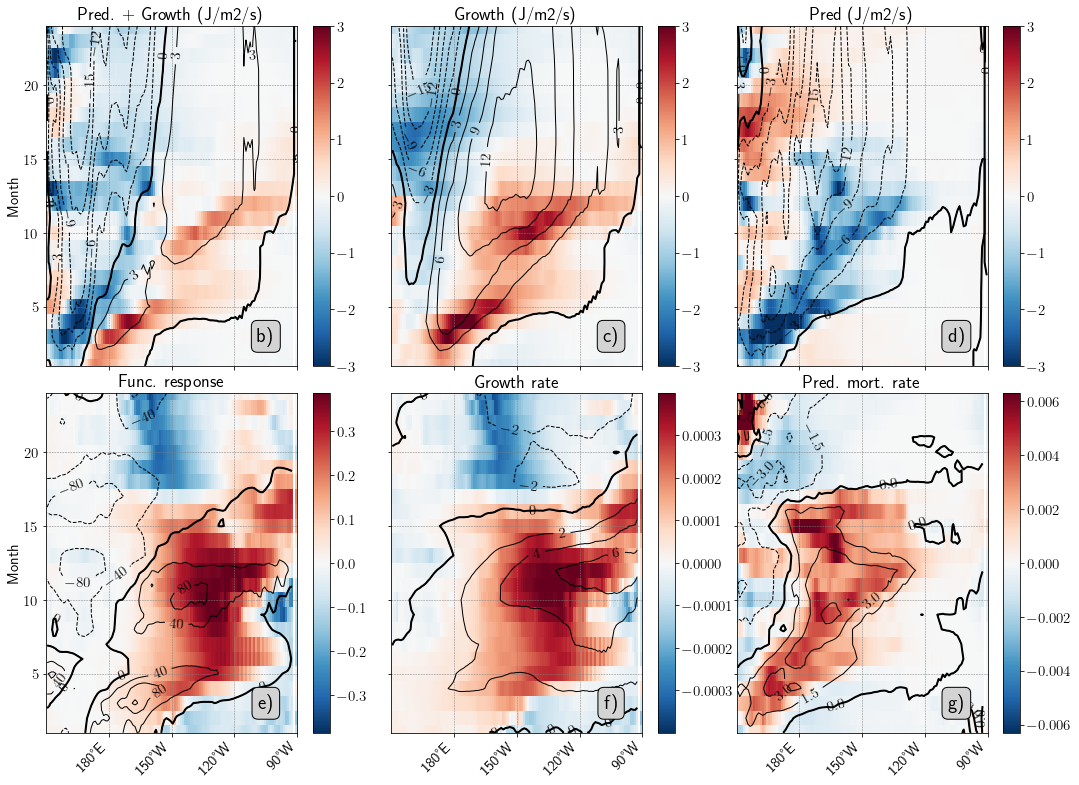
\includegraphics[scale=0.4]{figs/fig9.png}	
	\caption{Intermediate sizes trends (colors) and time-integrated trends (contours) for growth and predation (a and b). Growth rate (colors) and temperature (contours) anomalies (c). Predation mortality rate (colors) and large biomass anomalies (d). Functional response (colors) and small biomass (contours) anomalies (f).}	
	\label{fig:fig9}
\end{figure}

For large sizes, changes in fish biomass is dominated by advection/diffusion processes, while predation and growth have barely no impact. The possible reason is that as size increases, biological processes tend to be slower (\warn{is it true?}). Therefore, the biological response of large sizes to interannual events don't have necessary time to set-up. As a consequence, the interannual variability is solely driven by fish movements.

ADD HERE A SMALL PARAGRAPH SUMMARIZING THE DOMINANT PROCESSES DRIVING BIOMASS SHIFT FOR ALL SIZE CLASSES.

\subsection{subsurface response}

Figure \ref{fig:profiles} shows the mean equatorial profiles for temperature, zonal velocity, low-trophic level concentration and fish-biomass (contour lines) and the composites of OND El Nino anomalies. Mean temperature shows a deep thermocline in the western Pacific and a shallow one in the east, which flattens during El Nino conditions, hence leading to a warming in the east and a cooling in the west. The structure of the Equatorial Undercurrent is well visible on the zonal velocity profile. It strongly weakens during El Nino conditions, while strong positive (i.e. eastward) anomalies occur near the surface. Low-trophic level concentrations are maximum in the top 50m of the eastern Pacific and decrease during El Nino conditions, due to the flattening of the thermocline, which is associated with a decrease in nutrient supply.

Right columns of Fig \ref{fig:profiles} show the equatorial profiles of fish biomass density for the three size-classes. On average, biomass in the western Pacific reaches $100m$, while in the eastern Pacific, it remains very close to the surface $25m$. The western biomass for small sizes is maximal close at the surface close to the dateline, while for intermediate and large sizes, the maximum occurs at $50m$ in the western Pacific (between 150 and 160\degree{}E)
During El Nino conditions, fish biomass shows an increase in the eastern Pacific (except very close to the surface) and a decrease in the west. However, the latter is not homogeneous on the vertical, since positive anomalies are located at around 50m in the east for intermediate and large sizes. These anomalies are induced by a tightening of the vertical habitat, due to the thermocline flattening, which in turn modifies the vertical distribution of fish biomass.

\begin{figure}[h!tp]
	\centering
	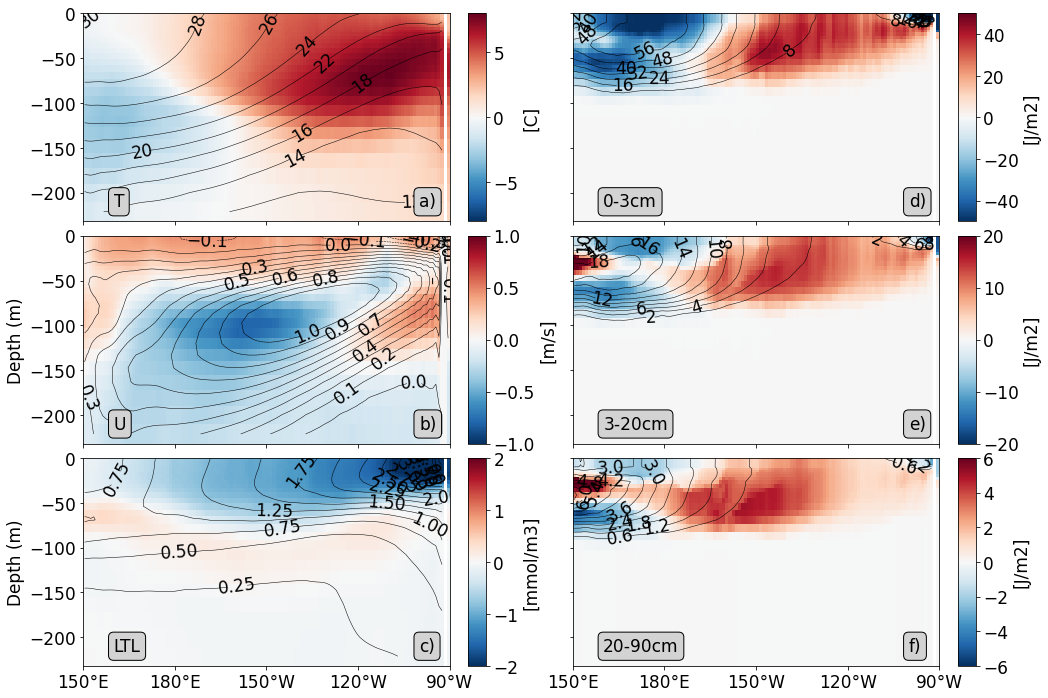
\includegraphics[scale=0.4]{figs/forage_mean_ond97.png}	
	\caption{Pacific equatorial profiles of temperature (a), zonal velocity (b), low-trophic concentration (c) and fish biomass (d for small, e for intermediate and f for large sizes). Mean are represented as black contour lines and El Nino anomalies are represented in colors.}	
	\label{fig:profiles}
\end{figure}

\subsection{Generalization}

Left column of Fig\ref{fig:mean_ond97_ape} shows the October, November and December composites of fish biomass density anomalies (colors), to which the climatological mean is superimposed (black contours). On average, fish biomass for small epipelagics is maximal at around 5\degree{}N and 5\degree{}S (see the $2.0$ contour on Fig \ref{fig:mean_ond97_ape}a), while smaller biomass is found at the equator and in the eastern Pacific. During El Nino conditions, biomass anomalies superimposes over the mean states, which may indicate an equatorward and an eastward shift of biomass location.
As size increases, the location of the biomass minimum on the central eastern Pacific extends westward and poleward, while the positive anomalies associated with El Nino conditions follow the same pattern: for intermediate sizes (Fig\ref{fig:mean_ond97_ape}b), the positive anomalies reach 180\degree{}E, while for small sizes, the anomalies are located east of 150\degree{}W. 

\begin{figure}[h!tp]
	\centering
	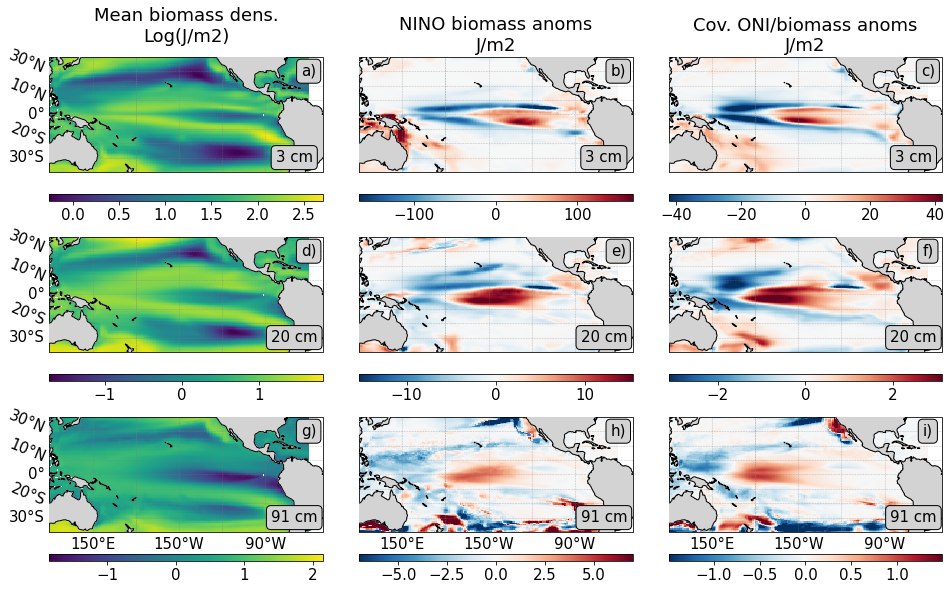
\includegraphics[scale=0.4]{figs/map_mean_anom_OND_97.png}	
	\caption{OND-NINO anomalies (left column) and covariance of fish biomass anomalies with the ONI index (right column) for small (upper line), intermediate (middle line) and large sizes (lower line). Black contours show the contours of mean fish biomass density (log-scale).}	
	\label{fig:mean_ond97_ape}
\end{figure}

%The patterns of the functional response and growth rates are very different for small sizes (figures YYY.a and YYY.d). The former shows negative anomalies on the central Pacific during the onset of El Nino conditions, presumably due to the concomitant reduction of plankton concentration (figure YYY.b). Interestingly, no anomalies are found in the eastern basin, due to compensating effects of warming temperatures and reduced plankton concentrations. The growth rate shows a pattern that is very similar to the temperature anomalies (Fig. XXX.a), indicating the dominance of temperature on the growth rate. The mortality rate (Fig. YYY.g) shows a pattern that is consistent with the increased biomass of intermediate epipelagics (XXX.b), which predate on small ones.  Besides, growth rate anomalies superimpose well on the small biomass anomalies (black contours in Fig. YYY.d), hence suggesting that the increased biomass during the El Nino conditions is triggered by enhanced growth associated with warmer temperature, despite a dampening effect of increased mortality rates.
%For intermediate sizes, the functional response and the growth rate show very similar anomalies, hence suggesting that they both are driven by the same factors. Both show positive anomalies during the onset of El Nino between 200E and 250E, presumably induced by the temperature warming that favours both the growth and search rates. Then negative anomalies occur, which are westward shifted relative to the positive ones. These negative anomalies are likely induced by the cooling associated with the La Nina conditions reinforced by the reduced small fish biomass that appears near 200E, as shown in Fig. XXX.d. Mortality rates anomalies are consistent with the increase of large fish biomass (Fig. XXX.f). Comparing the different fields, we can suggest that the increased fish biomass that appears on the central Pacific in early 1997 is first dominated by advective processes, which returns a similar pattern (fig YYY.k). Then, during the El Nino peak, the increased biomass of intermediate fish is driven by both an increased growth rate and an increased functional response, which are induced by warmer temperatures and more food available (more small epipelagic fishes, Fig. XXX.d).

%\subsection{Generalisation}
%
%In order to see if ecosystem response to the 97 El Nino event is representative, the covariance between fish biomass anomalies and the ONI index have been computed, following the methodology described in section \ref{sec:cov}. The maps are presented in Fig\ref{fig:ape_cov}.
%
%\begin{figure}
%	\centering
%	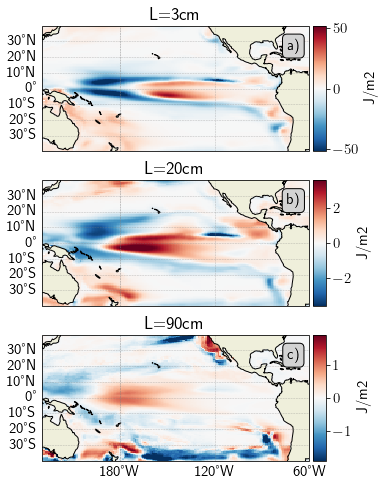
\includegraphics[scale=0.6]{figs/fig7.png}	
%	\caption{Covariance maps between the ONI index and the vertically integrated fish biomass anomalies for small (a), intermediate (b) and large (c) sizes.}	
%	\label{fig:ape_cov}
%\end{figure}
%
%The covariance patterns are very similar to the biomass anomalies depicted in Fig\ref{fig:mean_ond97_ape}, therefore suggesting that the mechanisms described in the above  apply to the general case. However, we note that the covariance patterns are westward shifted compared to the fish biomass anomalies. 
%
%This westward shift might be explained by the fact that when performing covariance anomalies, different El Nino events (Easter Pacific El Nino, Central Pacific El Nino) and La Nina events are considered, which ultimately impacts the global view of fish biomass response to ENSO variability.


%In this section, the interannual response of epipelagics to ENSO variability is investigated using covariance analysis. The left panels of Figure 3. show the yearly mean vertically integrated fish biomass over the entire simulation for the three different size classes. For small sizes (Figure 3a), the fish biomass is concentrated at around 10° S and 10 ° N in the central Pacific and close to the equator in the western Pacific. High biomass concentration is also found east of 90° W, off the coasts of Chile. As size increases, the equatorial "blue spot" extends meridionnally and to the west. This pattern is mostly driven by the active and passive advection of fishes in the Apecosm model (REF). Without advection, the biomass will be concentrated at the equator, where the plankton concentration is the maximum.
%
%Covariance maps between vertically integrated fish biomass and the winter ONI index are shown in the right panels of Figure 3. Small epipelagics show negative anomalies in the Western Equatorial Pacific and positive anomalies in the Central Equatorial Pacific. This pattern can be interpreted as an eastern displacement of the mean biomass in the Western Pacific. Similar dipolar patterns are also obtained for intermediate and large sizes, but the anomalies westward shifted as size increases. This can be interpreted, as for small sizes, by a westward shift of fish biomass during positive El Niño phases. The same results have been obtained when the covariance analysis is performed on monthly anomalies (not shown).


In order to insure that the extreme El Nino composites give a robust view of fish biomass response to ENSO variability, covariance maps are computed between the monthly ONI index and the detrended fish biomass anomalies over the 1958-2018 period (right column of Fig\ref{fig:mean_ond97_ape}). The El Nino composites and the covariance maps are very similar, despite westward shifted anomalies and lower amplitudes for the covariance maps compared to the composites. These  differences are due to the fact that covariance analysis includes Central Pacific (i.e. Modoki) El Nino events (such as the 1986, 1991, 1994, 2002, 2004 and 2009 events) and La Nina events, whose signature is not opposite to Eastern Pacific events. Nevertheless, the general agreement between the covariance maps and the El Nino composites suggest that the focus on the three major events gives a general view of fish biomass response to ENSO.